\documentclass[11pt,a4paper,sans]{moderncv}

\moderncvstyle{classic}
\moderncvcolor{blue}

% Show first and last name with the same weight for a more balanced title.
\renewcommand*{\namefont}{\fontsize{30}{32}\mdseries\upshape}
\definecolor{softaccent}{RGB}{77, 136, 204}
\newcommand{\company}[1]{\textcolor{softaccent}{\textbf{#1}}}
\newcommand{\metric}[1]{\textcolor{softaccent}{\textbf{#1}}}
\let\oldsection\section
\renewcommand{\section}[1]{%
  \par\vspace{0.35em}%
  \noindent\color{black}\rule{\textwidth}{0.5pt}%
  \par\vspace{0.45em}%
  \oldsection{#1}%
  \vspace{0.25em}%
}
\let\oldcventry\cventry
\renewcommand*{\cventry}[6]{\oldcventry{#1}{#2}{#3}{#4}{#5}{#6}\vspace{0.35em}}
\renewcommand{\labelitemi}{{\color{black}\textbullet}}
% Decorative logo under the date column (image only, nothing for ATS to parse).
\newcommand{\datelogo}[4]{\parbox[t]{\hintscolumnwidth}{\raggedleft #1\\[0.45em]\hfill\includegraphics[width=#3,trim=#4,clip]{images/#2.png}}}
\newcommand{\customcvtitle}{%
  \begin{minipage}[c]{0.74\textwidth}
    {\namefont Muhammet Emin Balmuk\par}
    \vspace{0.25em}
    {\large\itshape Computer Engineering Student\par}
    \vspace{0.6em}
    {\small Maltepe/Istanbul, Turkey \textbar\ +90 533 365 6944 \textbar\ \href{mailto:eminblmk@gmail.com}{eminblmk@gmail.com}\par}
    \vspace{0.2em}
    {\small Website: \href{https://eminbalmuk.github.io}{eminbalmuk.github.io} \textbar\ LinkedIn: \href{https://www.linkedin.com/in/eminbalmuk}{eminbalmuk} \textbar\ GitHub: \href{https://github.com/eminbalmuk}{eminbalmuk}\par}
  \end{minipage}\hfill
  \begin{minipage}[c]{0.2\textwidth}
    \raggedleft
    \setlength{\fboxsep}{1.5pt}%
    \fcolorbox{gray!55}{white}{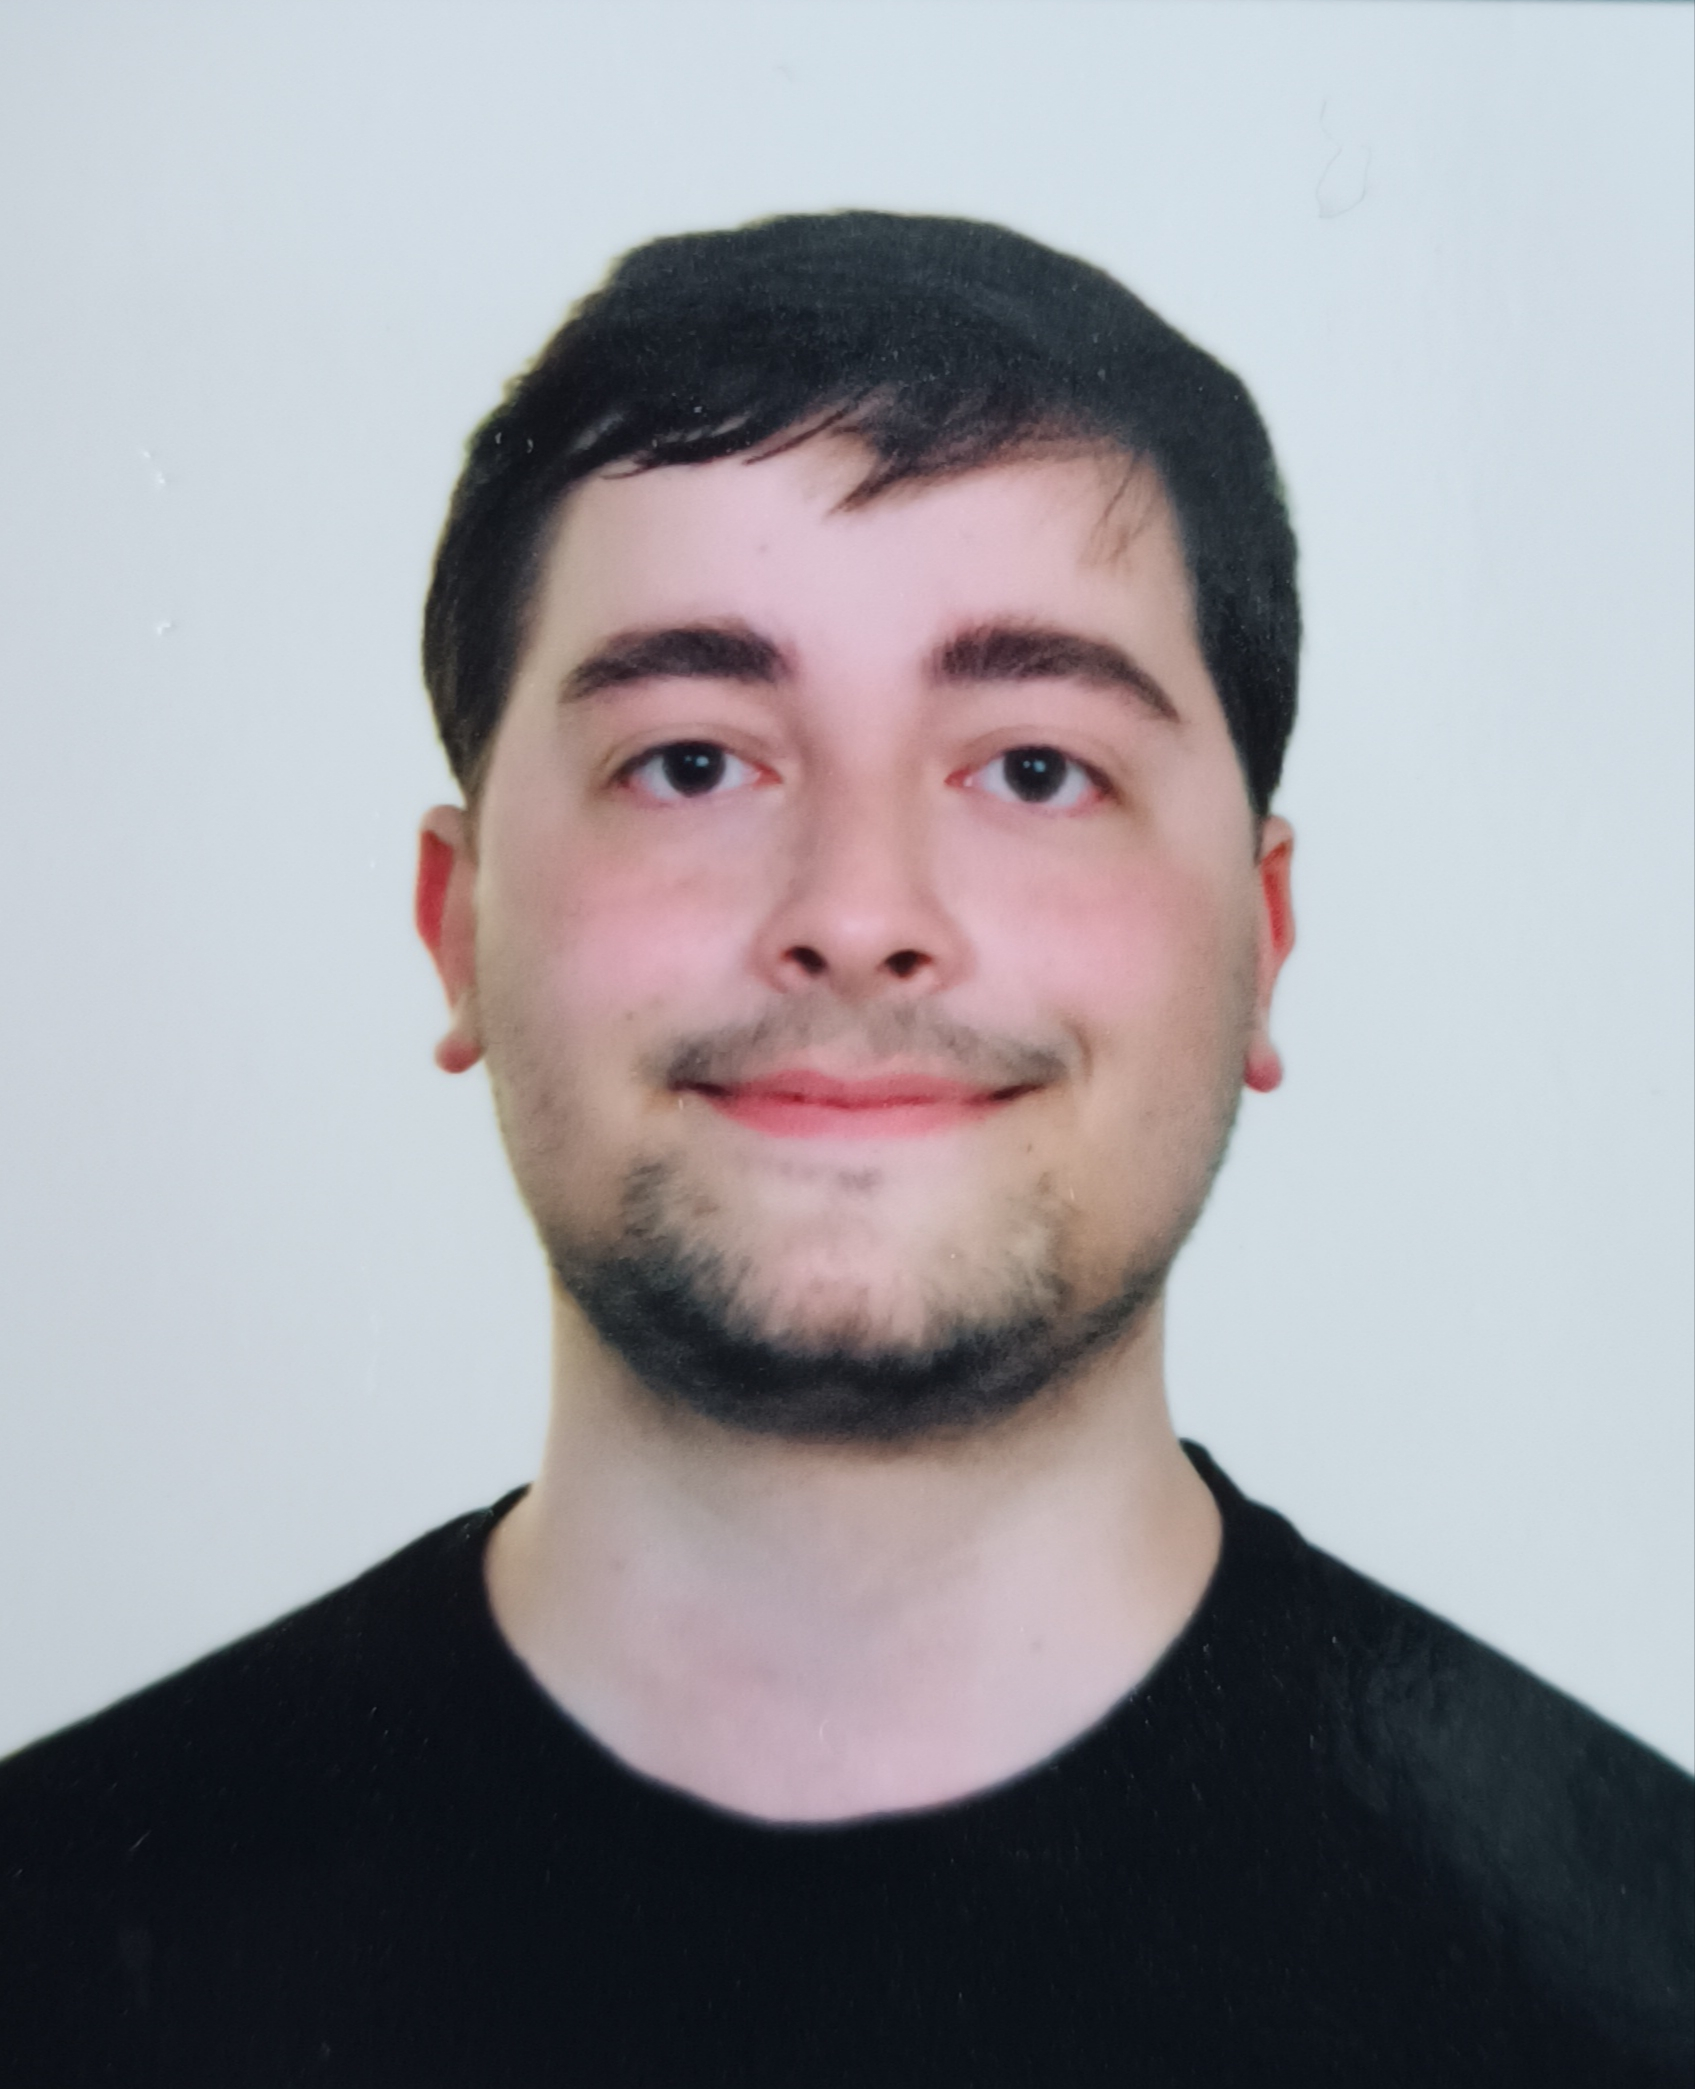
\includegraphics[width=0.93\linewidth]{images/profil.jpeg}}
  \end{minipage}
  \par\vspace{0.8em}
  \rule{\textwidth}{0.4pt}
  \par\vspace{0.6em}
}
\newcommand{\stackitem}[2]{%
  \cvitem{#1}{%
    \parbox[c]{0.6em}{\centering{\color{gray!55}\rule{0.35pt}{1.7\baselineskip}}}%
    \hspace{0.8em}%
    \parbox[t]{\dimexpr\linewidth-0.6em-0.8em\relax}{#2}%
  }%
}

\usepackage[scale=0.82, top=1.7cm, bottom=1.7cm]{geometry}
\usepackage[T1]{fontenc}
\usepackage[utf8]{inputenc}
\usepackage[english]{babel}
\usepackage{hyperref}
\usepackage{needspace}
\setlength{\hintscolumnwidth}{2.9cm}
\hypersetup{colorlinks=true, urlcolor=blue}

% PERSONAL INFORMATION
\name{Muhammet Emin Balmuk}
\title{}
\address{Maltepe/Istanbul}{Turkey}
\phone[mobile]{+90 533 365 6944}
\email{eminblmk@gmail.com}
\social[linkedin]{eminbalmuk}
\social[github]{eminbalmuk}

% Kept disabled in the ATS-friendly main version.
% You can uncomment the line below and add your own image file if needed.
\photo[64pt][0.4pt]{images/profil.jpeg}

\nopagenumbers{}

\begin{document}
\customcvtitle
\vspace{-0.4em}

\section{Profile}
Computer Engineering student at Marmara University, Co-founder \& CTO of \company{Giyiver} (a clothing-swap startup backed by investment received through Shell ILERIDE) and AI Engineering Intern at Orion Innovation, building LLM, vision-language, retrieval and speech AI systems. Solid experience in Python, machine learning and model evaluation from industry work, the Google AI and Technology Academy and personal projects. I enjoy turning models into reliable, measurable products.

\section{Education}
\cventry{2023 - 2027}{B.Sc. in Computer Engineering}{Marmara University}{Istanbul}{}{Third-year student}
\cventry{2019 - 2023}{High School}{Bah\c{c}elievler Anatolian High School (German)}{}{}{}

\section{Experience}
\cventry{\datelogo{June 2026 - Present}{giyiver}{1.1cm}{45 20 45 20}}{Co-founder \& CTO}{\company{Giyiver}}{Istanbul, \href{https://giyiverr.com}{giyiverr.com}}{}{
Turkish clothing-swap marketplace (barter, donation, points) live at \href{https://giyiverr.com}{giyiverr.com}. Backed by investment received through Shell ILERIDE. We are a team of 7, and I am responsible for the entire technical side of the project: web, mobile, backend, infrastructure, AI, security and testing.
\begin{itemize}
    \item \textbf{AI listing autofill:} a vision-language model (NVIDIA NIM, \metric{Nemotron 3.5 Super VL}) turns uploaded photos into title, category, colour, condition and description; images are downscaled client-side and sent as validated base64, so nothing is stored before publishing.
    \item \textbf{Model selection and hedged inference:} benchmarked candidate VLMs on real listing photos, dropped unreliable ones, disabled reasoning mode for \metric{2-10 s} typical latency, and added a fallback model that races the primary after 12 s (first valid answer wins, the loser is cancelled).
    \item \textbf{Multimodal moderation:} one VLM call checks all photos and text of a listing (real clothing, same item in every photo, consistent description); free text also passes a local profanity filter and an AI check, built to fail open and backed by database triggers.
    \item \textbf{Verified-image tokens:} HMAC-signed, user-bound tokens carry SHA-256 digests of the analysed images; at publish time the server re-hashes the uploaded files and skips the second VLM call only if every digest matches, saving latency and cost without trusting the client.
    \item \textbf{Platform:} Next.js on Cloudflare Pages with edge functions, Supabase Postgres with row-level security (\metric{57} migrations) and server-side points escrow, an Expo/React Native app, crawler-only rendering for SEO, and \metric{570+} automated tests including SQL tests on a real Postgres engine.
\end{itemize}}

\cventry{\datelogo{July 2026 - Present}{orion}{2.3cm}{40 155 55 155}}{AI Engineering Intern}{\company{Orion Innovation}}{Istanbul}{}{
Building LLM, retrieval and speech systems across three projects: \textbf{SOSIS} (Software product line Optimization for Safety-/mission-critical Industrial Systems, ITEA 4), an AI-driven test management platform; \textbf{GENIUS} (Generative AI for the Software Development Life Cycle), LLM-based requirement extraction; and \textbf{CLEAR} (Call Listener Emergency Audio Recognition), real-time audio intelligence for emergency call centers.
\begin{itemize}
    \item \textbf{SOSIS:} Designed a hybrid retrieval pipeline (dense embeddings + BM25, reciprocal rank fusion, GraphRAG) with optional listwise \metric{LLM reranking} that links requirements, tests and source code automatically.
    \item Benchmarked \metric{20+ LLMs} across 5 providers and \metric{10+ embedding models} on hand-labeled gold sets with paired bootstrap confidence intervals, reaching \metric{MRR 0.71} (requirement-to-test) and \metric{Hit@5 97.5\%} (test-to-code); wrote the study up as a research paper.
    \item Built an LLM pipeline that turns requirements into runnable Playwright tests, grounded with retrieved code, a graph-based page selector (page@3 \metric{63\%$\rightarrow$90\%}) and a headless-browser probe of the live UI, plus checks that feed the model its own mistakes back before the first run.
    \item Built LLM agents that adapt tests to a product variant, run them, repair failures from the run report and review the outcome (LLM-as-a-judge); mapped requirements to variants with a hybrid embedding scorer (\metric{F1 0.74}).
    \item Unified OpenRouter, NVIDIA NIM, Groq and Google AI Studio behind one client with provider routing, price caps and a token-per-minute scheduler.
    \item \textbf{GENIUS:} Optimized the multi-stage LLM requirement-extraction pipeline by batching zone classification, query expansion and rationale generation: LLM requests per document fell from \metric{95 to 9} (zone classification \metric{107 s$\rightarrow$3 s}, now well inside Groq's rate limit), and controlling reasoning effort on GLM 5.3 Flash halved token use (\metric{336K$\rightarrow$165K}).
    \item Evaluated the extracted requirements against a hand-written ground truth (\metric{12 of 18} items matched fully, 6 partially, none missed), and integrated GENIUS into SOSIS so that its EARS/LESS requirements and labels (ISO 25010 quality dimension, actor, classification) feed test generation and variant mapping.
    \item \textbf{CLEAR:} Built a streaming pipeline that runs speech recognition (Qwen3-ASR with LoRA), speaker diarization, speech emotion, stress and audio-event models on live 911/112 calls, fully on-premise on CPU.
    \item Trained calibrated accent classifiers on Whisper encoder features and combined emotion and stress signals for distress detection (\metric{AUROC 0.87} vs 0.71 for stress alone).
    \item Evaluated models on public benchmarks: \metric{6.3\%} WER on clean speech, \metric{86\%} emotion accuracy (vs \metric{41\%} for the earlier approach), first words appear on screen in about \metric{2 s}.
\end{itemize}}

\cventry{\datelogo{January 2026 - Present}{gdg}{1.9cm}{390 740 390 740}}{AI Team Lead}{\company{GDG - Google Developer Group Marmara}}{}{}{
\begin{itemize}
    \item Lead the AI team at GDG Marmara, driving technical projects and developer-focused community activities.
    \item Work with the team on project planning, product thinking and delivery for software projects and community events.
    \item Help turn ideas into buildable projects while building coordination, ownership and community skills.
\end{itemize}}

\cventry{\datelogo{February 2026 - June 2026}{shell}{1.1cm}{100 20 100 20}}{ILERIDE Program \textbar\ Trainee \& Startup Founder}{\company{Shell}}{Istanbul}{}{
\begin{itemize}
    \item Took part in Shell's ILERIDE program, which focused on structured thinking, problem framing, communication and business skills.
    \item \textbf{Giyiver}, the startup I co-founded and lead as CTO, \metric{received investment} through the program.
    \item Used what I learned in the program for Giyiver's product and technical decisions, and to explain technical work to non-technical people.
\end{itemize}}

\cventry{\datelogo{December 2024 - August 2025}{yzta}{1.1cm}{290 185 295 180}}{Data Science Trainee}{\company{Google AI and Technology Academy}}{Istanbul}{}{
\begin{itemize}
    \item Completed an intensive 8-month program in applied data science, machine learning and end-to-end project development.
    \item Learned to work with real datasets, from analysis and statistics to model evaluation and turning results into insights, through coursework and team projects.
    \item Took part in datathons and bootcamps, building models and working in teams under tight deadlines.
    \item Helped build an AI-supported mobile app for preliminary dementia assessment during the bootcamp, finishing \metric{3rd among 205 teams}.
\end{itemize}}

\needspace{8\baselineskip}
\section{Projects}

\cventry{2026}{Credit Card Fraud Detection System}{Personal Project}{}{}{
\begin{itemize}
    \item Developed a production-ready machine learning pipeline for fraud detection using a dataset of \metric{1.04M+ transactions}.
    \item Implemented \metric{leakage-free feature engineering} using point-in-time calculations (velocity, behavioral patterns) to prevent future data leakage.
    \item Optimized and compared LightGBM, XGBoost, CatBoost, and Random Forest models, achieving a \metric{0.925 PR-AUC} and \metric{0.85 F1-Score}.
    \item Addressed extreme class imbalance (\metric{0.58\% fraud}) by prioritizing Precision-Recall AUC optimization to minimize false positives in a financial context.
    \item Built automated diagnostic tools for data distribution analysis and model performance visualization using Pandas, Matplotlib, and Seaborn.
    \item \href{https://github.com/eminbalmuk/fraud-detection-ml}{GitHub Repository}
\end{itemize}}

\cventry{2026}{Unsolved: AI-Driven Problem Discovery Platform \& Automated Scraper}{Personal Project}{}{}{
\begin{itemize}
    \item Built an automated research pipeline with \metric{Next.js 16} and \metric{TypeScript} that scrapes real-time customer signals from \metric{Reddit API} and \metric{App Store RSS} feeds to identify unaddressed needs and market gaps.
    \item Developed a heuristic scoring engine that analyzes raw text signals using \metric{keyword-based NLP} and sentiment weights to quantify \metric{Pain Intensity}, \metric{Frequency}, and \metric{Willingness to Pay (WTP)}.
    \item Built an ingestion layer with \metric{deduplication logic} and \metric{automatic categorization} (Bug, Feature Request, Experience Gap), transforming thousands of raw social signals into actionable product insights.
    \item Added a persistence layer with \metric{Prisma ORM} and \metric{PostgreSQL}, featuring \metric{upsert mechanisms} to maintain a synchronized "Problem Store" that tracks market trends and competitor gaps over time.
    \item Integrated an \metric{AI Analysis Engine} that utilizes custom prompt versioning to generate structured product strategy reports, including MVP steps, solution ideas, and risk assessments based on ingested market signals.
    \item \href{https://github.com/eminbalmuk/Unsolved-AI}{GitHub Repository}
\end{itemize}}

\cventry{2026}{TaskFlow Collaborative Kanban Platform}{Personal Project}{}{}{
\begin{itemize}
    \item Built a full-stack Kanban board application with \metric{Next.js}, \metric{React}, \metric{TypeScript}, \metric{Prisma}, and \metric{PostgreSQL}, focused on practical team task management.
    \item Developed responsive dashboard and landing page flows, including drag-and-drop board interactions, due dates, multi-assignee task management, and mobile-friendly board navigation.
    \item Implemented \metric{role-based collaboration} features such as board sharing, viewer/editor permissions, self-leave flows for invited users, and access-aware UI/route protection.
    \item Designed and maintained API routes, database schema migrations, and state management for real-time-feeling collaborative workflows across shared boards.
    \item \href{https://github.com/eminbalmuk/taskflow-kanban}{GitHub Repository}
\end{itemize}}

\cventry{2025}{Crypto Analysis and Trading Bot}{Personal Project}{}{}{
\begin{itemize}
    \item Built a Python trading bot based on custom quantitative strategies.
    \item Designed an architecture that screens \metric{200+ crypto assets} in about \metric{2 minutes} and reached a \metric{66\% success rate} with a \metric{1:2.5 risk-reward ratio} in a real-time Telegram signal system.
    \item Evaluated LightGBM, CatBoost, and TabNet during R\&D, then refactored the live system into a custom strategy-based architecture to reduce latency.
    \item Processed high-volume market data with NumPy and Pandas and maintained trade logs and historical records in MongoDB.
    \item Automated 24/7 trade lifecycle tracking through an additional ``Crypto Signal Tracker'' bot.
\end{itemize}}

\cventry{2025}{Datathon Competition}{Google AI and Technology Academy}{}{}{
\begin{itemize}
    \item Led the data analysis and visualization of a \metric{210,000-row dataset} in a \metric{4-person cross-functional team}.
    \item Built price prediction models for a new \metric{56,000-row dataset} using LightGBM, Random Forest, and XGBoost.
    \item Interpreted model outputs and translated complex findings into actionable visual insights with Matplotlib and Seaborn.
\end{itemize}}

\cventry{2025}{AI-Integrated Health Application}{Bootcamp Project}{}{}{
\begin{itemize}
    \item Developed a mobile application with a \metric{5-person team} for the preliminary assessment of cognitive conditions such as hyperactivity, dementia, and autism.
    \item Developed the Python backend and core Dart frontend components, leading the team to rank in the \metric{top 3 among 205 competing teams}.
    \item Architected a voice pronunciation test module in Python, managed Firebase operations, and integrated systems through REST APIs.
    \item Optimized several Dart screens and fixed critical security vulnerabilities.
    \item \href{https://github.com/BBBeyza/YZTA_YapayZeka_Grup-132}{GitHub Repository}
\end{itemize}}

\cventry{2025}{Fire Detection System for Live Security Cameras}{Computer Vision}{}{}{
\begin{itemize}
    \item Trained a model on a dataset of \metric{95,000 images} using YOLO 11.
    \item Reached \metric{82.8\%} smoke detection accuracy and \metric{79.6\%} fire detection accuracy, with especially strong results on black-and-white images.
    \item Tested the system on both live camera streams and recorded video footage, marking detected regions with bounding boxes.
    \item \href{https://github.com/eminbalmuk/yolo-fire-and-smoke-detection}{GitHub Repository}
\end{itemize}}

\cventry{2025}{Real-Time Chat Application}{Team Project}{}{}{
\begin{itemize}
    \item Built a real-time messaging application with a 3-person team using HTML, CSS (Tailwind), JavaScript, React, Node.js, MongoDB, and Socket.io.
    \item Managed Node.js backend tasks, real-time connection management with Socket.io, MongoDB workflows, and media storage with Cloudinary.
\end{itemize}}

\cventry{2024}{Automated Linux Backup System}{Personal Project}{}{}{
\begin{itemize}
    \item Engineered a modular \metric{Bash-based backup system} with support for both interactive TUI and fully automated headless execution modes.
    \item Integrated a dynamic terminal-based file explorer and user interface using the \metric{dialog} library to enhance user experience.
    \item Ensured data security through \metric{atomic scheduling via crontab}, recursive file management with find, and optimized archive compression using tar.
    \item Implemented a centralized logging mechanism to provide end-to-end traceability and auditability of backup operations.
\end{itemize}}

\cventry{2024}{Energy Distribution and Fault Response Simulation}{Team Project}{}{}{
\begin{itemize}
    \item Built a city-scale energy fault simulation using Spring Boot and JavaScript to model real-time detection and response workflows for urban power outages.
    \item Designed the full JavaScript/HTML interface and supported backend integration for optimized outage-response workflows.
\end{itemize}}

\cventry{2024}{Personal Series/Movie Watchlist Platform}{Team Project}{}{}{
\begin{itemize}
    \item Developed a social watchlist application using Python (backend) and CustomTkinter (frontend) within a 3-person team.
    \item Engineered core backend features and designed the RESTful API layer to ensure seamless communication between system components.
    \item End-to-end feature development including personal watchlist management and social interaction modules.
\end{itemize}}

\section{Technical Skills}
\stackitem{Programming Languages}{Python, TypeScript, JavaScript, Java, C/C++, Dart, Bash}
\stackitem{LLM Engineering}{LLM agents, LLM-as-a-judge, structured output, prompt engineering, reasoning-effort control, request batching, multi-provider routing and rate-limit scheduling (OpenRouter, NVIDIA NIM, Groq, Google AI Studio)}
\stackitem{Retrieval and RAG}{Hybrid search (BM25 + dense embeddings), score fusion (RRF, DBSF), GraphRAG, listwise LLM reranking, query expansion, sentence-transformers, Qdrant}
\stackitem{Multimodal and Vision}{Vision-language models (Nemotron VL), multimodal content moderation, VLM benchmarking and fallback inference, YOLO object detection}
\stackitem{Speech and Audio}{Speech recognition (Qwen3-ASR, Whisper), LoRA fine-tuning, speaker diarization, speech emotion recognition (wav2vec 2.0, emotion2vec), stress and audio-event detection, real-time streaming, on-premise CPU inference}
\stackitem{Machine Learning}{PyTorch, scikit-learn, LightGBM, XGBoost, CatBoost, TabNet, Keras, Pandas, NumPy, Matplotlib, Seaborn}
\stackitem{Model Evaluation}{Hand-labeled gold sets, MRR, Hit@k, paired bootstrap confidence intervals, WER, AUROC, PR-AUC, F1, probability calibration}
\stackitem{Web and Mobile}{FastAPI, Next.js, React, Node.js, Expo / React Native, Spring Boot, REST, WebSocket, Socket.io}
\stackitem{Data and DevOps}{PostgreSQL, Supabase, MongoDB, Prisma, Firebase, SQL / MSSQL, Docker, Cloudflare Pages, GitLab CI/CD, Playwright, pytest, Git, uv}

\section{Languages}
\cvitemwithcomment{Turkish}{Native}{}
\cvitemwithcomment{English}{B2}{}
\cvitemwithcomment{German}{A2-B1}{}

\section{Certificates}
\cvitem{2026}{Artificial Intelligence Specialization Program - Foundation Training Certificate (Republic of T\"urkiye Ministry of Industry and Technology)}
\cvitem{2026}{Introduction to Open Source License Compliance Management (The Linux Foundation)}
\cvitem{2026}{Model Context Protocol: Advanced Topics (Anthropic)}
\cvitem{2026}{AI Fluency: Framework \& Foundations (Anthropic)}
\cvitem{2026}{Claude 101 (Anthropic)}
\cvitem{2025}{Google AI and Technology Academy Graduation Certificate}
\cvitem{2025}{Bootcamp Finalist Certificate of Achievement (Google AI \& Technology Academy)}
\cvitem{2025}{Google Advanced Data Analytics Certificate}
\cvitem{2025}{Foundations of Data Science (Google)}
\cvitem{2025}{The Nuts and Bolts of Machine Learning}
\cvitem{2025}{Regression Analysis: Simplify Complex Data Relationships (Google)}
\cvitem{2025}{Go Beyond the Numbers: Translate Data into Insights (Google)}
\cvitem{2025}{The Power of Statistics (Google)}
\cvitem{2025}{Get Started with Python (Google)}
\cvitem{2025}{Foundations of Project Management (Google)}
\cvitem{2022}{Deutsches Sprachdiplom 1 (Kultusministerkonferenz)}

\end{document}
